\documentclass[aspectratio=169, 10pt]{beamer}

\usepackage{graphicx}
\usepackage{tabularx}
\usepackage{booktabs}
\usepackage{xcolor}
\usepackage{tikz}
\usepackage{listings}
\usepackage{mathptmx}
\usepackage{helvet}
\usepackage{array}
\usepackage{colortbl}
\usepackage{microtype}

% ─── Colors ───
\definecolor{darkred}{RGB}{178, 34, 34}
\definecolor{nithgold}{RGB}{204, 153, 51}
\definecolor{beamerblue}{RGB}{51, 51, 178}
\definecolor{codebg}{RGB}{30, 30, 46}
\definecolor{codegreen}{RGB}{80, 200, 120}
\definecolor{codeyellow}{RGB}{255, 213, 79}
\definecolor{codecyan}{RGB}{100, 210, 255}
\definecolor{codegray}{RGB}{160, 160, 160}

% ─── Beamer theme ───
\setbeamertemplate{navigation symbols}{}
\setbeamertemplate{itemize items}[triangle]
\setbeamercolor{item}{fg=beamerblue}
\setbeamercolor{subitem}{fg=darkred}
\setbeamercolor{subsubitem}{fg=nithgold}

% ─── Code listings ───
\lstset{
  backgroundcolor=\color{codebg},
  basicstyle=\ttfamily\scriptsize\color{white},
  keywordstyle=\color{codecyan}\bfseries,
  commentstyle=\color{codegray}\itshape,
  stringstyle=\color{codegreen},
  numberstyle=\tiny\color{codegray},
  breaklines=true,
  numbers=left,
  numbersep=5pt,
  frame=single,
  framerule=0pt,
  xleftmargin=8pt,
  xrightmargin=4pt,
  aboveskip=3pt,
  belowskip=3pt,
}

% ─── Title page ───
\defbeamertemplate*{title page}{customized}[1][]
{
  \begin{center}
    \vspace{0.2cm}
    \textbf{\large \rmfamily Smart Vaccine Delivery System} \\
    \vspace{0.1cm}
    \textcolor{darkred}{\textbf{\normalsize \rmfamily IoT-Based Cold-Chain Monitoring \& Safety Analytics}} \\
    \vspace{0.4cm}
    {\small Course EC-308: Internet of Things} \\
    \vspace{0.4cm}
    \begin{columns}
      \begin{column}{0.35\textwidth}
        \begin{flushleft}\small
          Presented to:\\
          Dr.\ [Professor Name]
        \end{flushleft}
      \end{column}
      \begin{column}{0.3\textwidth}
        \begin{center}
          
\includegraphics[width=2.3cm]{nith_logo.png}
        \end{center}
      \end{column}
      \begin{column}{0.35\textwidth}
        \begin{flushright}\small
          Presented By:\\
          Anirudh Sharma\\
          Roll No: 22DCS002
        \end{flushright}
      \end{column}
    \end{columns}
    \vspace{0.4cm}
    {\small BTech DD 8\textsuperscript{th} Semester, 2025--26}\\
    \vspace{0.1cm}
    \textbf{\small Department of Computer Science and Engineering}\\
    \textbf{\small National Institute of Technology Hamirpur}
  \end{center}
}

% ─── Frame title ───
\setbeamertemplate{frametitle}{
    \vspace{0.4cm}
    \begin{columns}[c]
    \begin{column}{0.85\textwidth}
        \textbf{\textcolor{darkred}{\Large \rmfamily \insertframetitle}}
    \end{column}
    \begin{column}{0.15\textwidth}
        \begin{flushright}
            \vspace{-0.2cm}
            
\includegraphics[height=0.85cm]{nith_logo.png}\hspace*{-0.3cm}
        \end{flushright}
    \end{column}
    \end{columns}
    \vspace{0.1cm}
}

% ─── Footer ───
\setbeamertemplate{footline}{
    \leavevmode%
    \hbox{%
      \begin{beamercolorbox}[wd=0.6\paperwidth,ht=2.2ex,dp=1ex,left]{author in head/foot}%
        \hspace{0.3cm}\tiny\textcolor{nithgold}{Smart Vaccine Delivery System $|$ IoT Simulation}
      \end{beamercolorbox}%
      \begin{beamercolorbox}[wd=0.4\paperwidth,ht=2.2ex,dp=1ex,right]{title in head/foot}%
        \tiny \insertframenumber{} / \inserttotalframenumber\hspace*{0.3cm}
      \end{beamercolorbox}}%
    \vskip0pt%
}

% ─── Placeholder macro ───
\newcommand{\imgph}[3]{%
  \begin{tikzpicture}
    \draw[darkred, dashed, line width=1.2pt, rounded corners=5pt]
      (0,0) rectangle (#1,#2);
    \node[text=nithgold, font=\bfseries\small] at (#1/2,{#2/2+0.2}) {[\,Simulation Screenshot\,]};
    \node[text=codegray, font=\footnotesize\itshape] at (#1/2,{#2/2-0.2}) {#3};
  \end{tikzpicture}%
}

% reduce global line spacing slightly
\setlength{\itemsep}{0pt}

\begin{document}

%% ═════════════════════════════════════════
%%  1 — TITLE SLIDE
%% ═════════════════════════════════════════
\begin{frame}[plain]
  \titlepage
\end{frame}

%% ═════════════════════════════════════════
%%  2 — TABLE OF CONTENTS
%% ═════════════════════════════════════════
\begin{frame}{Table of Contents}
  \begin{columns}[t]
    \begin{column}{0.5\textwidth}
      \begin{itemize}\setlength\itemsep{0.38em}
        \item Introduction \& Problem Statement
        \item Limitations
        \item Proposed Solution
        \item Tools \& Sensors
          \begin{itemize}\setlength\itemsep{0.15em}
            \item Resistors \& Values
            \item Pin Mapping (GPIOs Used)
            \item Why These Components?
          \end{itemize}
        \item Simulation (Wokwi)
        \item Cloud Integration
      \end{itemize}
    \end{column}
    \begin{column}{0.5\textwidth}
      \begin{itemize}\setlength\itemsep{0.38em}
        \item Code Walkthrough
        \item Results
        \item Limitations
        \item Future Scope
        \item Conclusion
        \item References
      \end{itemize}
    \end{column}
  \end{columns}
\end{frame}

%% ═════════════════════════════════════════
%%  3 — INTRODUCTION & PROBLEM STATEMENT
%% ═════════════════════════════════════════
\begin{frame}[shrink=5]{Introduction \& Problem Statement}
  \begin{columns}[T]
    \begin{column}{0.58\textwidth}
      \textbf{\textcolor{darkred}{Background}}
      \begin{itemize}\setlength\itemsep{0.25em}
        \item Vaccines require strict cold-chain maintenance (2\textdegree C--8\textdegree C) during transport
        \item WHO reports up to \textbf{50\% vaccine wastage} due to cold-chain failures globally
        \item Manual monitoring is unreliable and lacks real-time alerts
        \item Physical damage (drops, vibration) and gas leakage go undetected
      \end{itemize}
      \vspace{0.35em}
      \textbf{\textcolor{darkred}{Problem Statement}}
      \begin{itemize}\setlength\itemsep{0.25em}
        \item How do we \textit{continuously} monitor temperature, humidity, mechanical stress, and contamination during vaccine transport?
        \item How do we \textit{automatically} raise alerts and log violations to the cloud in real time?
      \end{itemize}
    \end{column}
    \begin{column}{0.4\textwidth}
      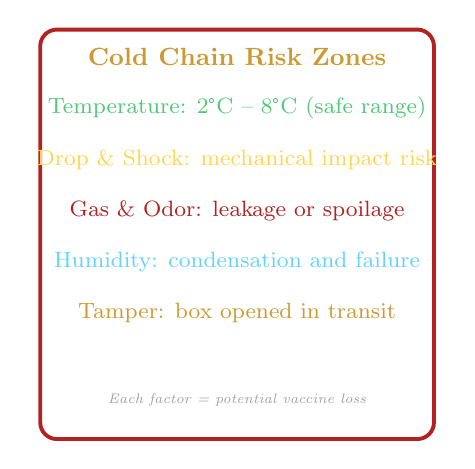
\begin{tikzpicture}[font=\footnotesize]
        \draw[darkred, line width=1.4pt, rounded corners=6pt]
          (0,0) rectangle (5.0,5.2);
        \node[text=nithgold, font=\bfseries\small] at (2.5,4.85) {Cold Chain Risk Zones};
        \node[text=codegreen]  at (2.5,4.20) {Temperature: 2\textdegree C -- 8\textdegree C (safe range)};
        \node[text=codeyellow] at (2.5,3.55) {Drop \& Shock: mechanical impact risk};
        \node[text=darkred]    at (2.5,2.90) {Gas \& Odor: leakage or spoilage};
        \node[text=codecyan]   at (2.5,2.25) {Humidity: condensation and failure};
        \node[text=nithgold]   at (2.5,1.60) {Tamper: box opened in transit};
        \node[text=codegray, font=\tiny\itshape] at (2.5,0.5) {Each factor = potential vaccine loss};
      \end{tikzpicture}
    \end{column}
  \end{columns}
\end{frame}

%% ═════════════════════════════════════════
%%  3b — LIMITATIONS
%% ═════════════════════════════════════════
\begin{frame}[shrink=2]{Limitations}
  \begin{columns}[T]
    \begin{column}{0.5\textwidth}
      \textbf{\textcolor{darkred}{Hardware / Simulation Constraints}}
      \begin{itemize}\setlength\itemsep{0.3em}
        \item \textbf{MPU6050 not in Wokwi} --- simulated via potentiometers; real I2C dynamics not fully represented
        \item \textbf{MQ-135 warm-up} --- requires 24--48\,hrs in real deployment; simulation is instantaneous
        \item \textbf{ESP32 ADC non-linearity} --- GPIO 34/35 accuracy is $\pm6$\% without calibration
        \item \textbf{ThingSpeak free-tier} --- 15\,s minimum upload interval; unsuitable for high-frequency events
      \end{itemize}
    \end{column}
    \begin{column}{0.5\textwidth}
      \textbf{\textcolor{darkred}{System-Level Limitations}}
      \begin{itemize}\setlength\itemsep{0.3em}
        \item \textbf{No GPS} --- violation location unknown; route safety analysis not possible
        \item \textbf{No power management} --- continuous WiFi drains battery; external power needed for long trips
        \item \textbf{No encryption} --- API key hardcoded; vulnerable if network is intercepted
        \item \textbf{Single point of failure} --- one ESP32 failure stops all monitoring; no redundancy
        \item \textbf{WiFi only} --- no offline buffering; data lost on connectivity drop
      \end{itemize}
    \end{column}
  \end{columns}
\end{frame}

%% ═════════════════════════════════════════
%%  4 — PROPOSED SOLUTION
%% ═════════════════════════════════════════
\begin{frame}[shrink=3]{Proposed Solution}
  \begin{columns}[T]
    \begin{column}{0.57\textwidth}
      \textbf{\textcolor{darkred}{System Architecture}}
      \begin{itemize}\setlength\itemsep{0.28em}
        \item \textbf{ESP32} MCU with built-in WiFi for edge processing \& cloud upload
        \item \textbf{DHT22} — Temperature + Humidity (cold-chain \& condensation)
        \item \textbf{MPU6050} — Accelerometer + Gyroscope (shock, drop, rash driving)
        \item \textbf{MQ-135} — Gas sensor (leakage / spoilage detection)
        \item \textbf{Tamper switch} — Physical security of vaccine box
        \item \textbf{Buzzer + LED} — Immediate on-device alerts
        \item \textbf{ThingSpeak} — Cloud logging with 8-field data channel
        \item \textbf{Web Dashboard} — Real-time gauges, charts, event simulation
      \end{itemize}
    \end{column}
    \begin{column}{0.41\textwidth}
      \begin{center}
      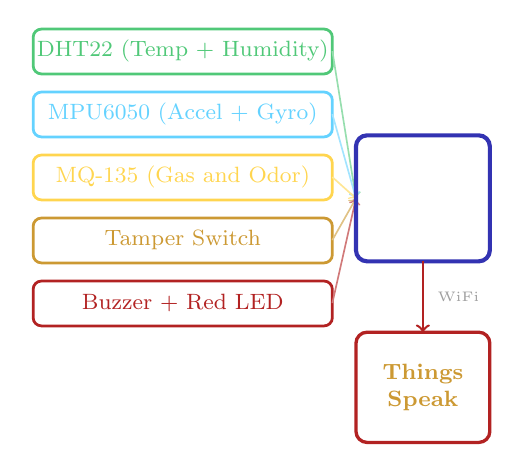
\begin{tikzpicture}[font=\small]
        % DHT22
        \draw[codegreen, line width=1pt, rounded corners=3pt] (0,5.18) rectangle (3.8,5.75);
        \node[text=codegreen, font=\footnotesize] at (1.9,5.47) {DHT22 (Temp + Humidity)};
        \draw[->, codegreen!60, line width=0.6pt] (3.8,5.47) -- (4.1,3.6);
        % MPU6050
        \draw[codecyan, line width=1pt, rounded corners=3pt] (0,4.38) rectangle (3.8,4.95);
        \node[text=codecyan, font=\footnotesize] at (1.9,4.67) {MPU6050 (Accel + Gyro)};
        \draw[->, codecyan!60, line width=0.6pt] (3.8,4.67) -- (4.1,3.6);
        % MQ-135
        \draw[codeyellow, line width=1pt, rounded corners=3pt] (0,3.58) rectangle (3.8,4.15);
        \node[text=codeyellow, font=\footnotesize] at (1.9,3.87) {MQ-135 (Gas and Odor)};
        \draw[->, codeyellow!60, line width=0.6pt] (3.8,3.87) -- (4.1,3.6);
        % Tamper Switch
        \draw[nithgold, line width=1pt, rounded corners=3pt] (0,2.78) rectangle (3.8,3.35);
        \node[text=nithgold, font=\footnotesize] at (1.9,3.07) {Tamper Switch};
        \draw[->, nithgold!60, line width=0.6pt] (3.8,3.07) -- (4.1,3.6);
        % Buzzer + LED
        \draw[darkred, line width=1pt, rounded corners=3pt] (0,1.98) rectangle (3.8,2.55);
        \node[text=darkred, font=\footnotesize] at (1.9,2.27) {Buzzer + Red LED};
        \draw[->, darkred!60, line width=0.6pt] (3.8,2.27) -- (4.1,3.6);
        % ESP32 box
        \draw[beamerblue, line width=1.5pt, rounded corners=4pt] (4.1,2.8) rectangle (5.8,4.4);
        \node[text=white, font=\bfseries\footnotesize, align=center] at (4.95,3.6) {ESP32\\DevKit};
        % ThingSpeak box
        \draw[darkred, line width=1.2pt, rounded corners=4pt] (4.1,0.5) rectangle (5.8,1.9);
        \node[text=nithgold, font=\bfseries\footnotesize, align=center] at (4.95,1.2) {Things\\Speak};
        \draw[->, darkred, line width=0.9pt] (4.95,2.8) -- (4.95,1.9);
        \node[text=codegray, font=\tiny] at (5.4,2.35) {WiFi};
      \end{tikzpicture}
      \end{center}
    \end{column}
  \end{columns}
\end{frame}

%% ═════════════════════════════════════════
%%  5 — TOOLS & SENSORS
%% ═════════════════════════════════════════
\begin{frame}[shrink=3]{Tools \& Sensors}
  \begin{columns}[T]
    \begin{column}{0.5\textwidth}
      \textbf{\textcolor{darkred}{Hardware Components}}
      \vspace{0.2em}
      {\small
      \begin{tabular}{@{}ll@{}}
        \toprule
        \textbf{Component} & \textbf{Purpose} \\
        \midrule
        ESP32 DevKit v4 & Main MCU + WiFi \\
        DHT22 & Temp \& Humidity sensing \\
        MPU6050 & Acceleration + Gyroscope \\
        MQ-135 & Gas / Odor detection \\
        Push Button & Tamper detection \\
        Passive Buzzer & Audible alarm \\
        Red LED & Visual alert indicator \\
        Resistor 4.7k$\Omega$ & DHT22 pull-up \\
        Resistor 220$\Omega$ & LED current limiter \\
        \bottomrule
      \end{tabular}
      }
    \end{column}
    \begin{column}{0.5\textwidth}
      \textbf{\textcolor{darkred}{Software \& Simulation Tools}}
      \begin{itemize}\setlength\itemsep{0.28em}
        \item \textbf{Wokwi} — Browser-based ESP32 simulation
        \item \textbf{Arduino C++} — Firmware development
        \item \textbf{DHTesp Library} — DHT22 driver
        \item \textbf{WiFi.h / HTTPClient.h} — Cloud comms
        \item \textbf{ThingSpeak} — IoT cloud data platform
        \item \textbf{HTML/CSS/JS + Chart.js} — Dashboard
      \end{itemize}
      \vspace{0.35em}
      \textbf{\textcolor{darkred}{Simulation Note}}
      \begin{itemize}\setlength\itemsep{0.2em}
        \item MPU6050 \& MQ-135 simulated via \textbf{potentiometers} in Wokwi (no hardware needed)
        \item Full I2C / analog code available for physical deployment
      \end{itemize}
    \end{column}
  \end{columns}
\end{frame}

%% ═════════════════════════════════════════
%%  5b — RESISTORS & PIN MAPPING
%% ═════════════════════════════════════════
\begin{frame}[shrink=3]{Tools \& Sensors --- Resistors \& Pin Mapping}
  \begin{columns}[T]
    \begin{column}{0.46\textwidth}
      \textbf{\textcolor{darkred}{Resistors Used}}
      \vspace{0.2em}
      {\small
      \begin{tabular}{@{}ccl@{}}
        \toprule
        \textbf{Ref.} & \textbf{Value} & \textbf{Purpose} \\
        \midrule
        R1 & 4700\,$\Omega$ & DHT22 pull-up to 3.3\,V \\
        R2 & 220\,$\Omega$ & LED current limiter \\
        \bottomrule
      \end{tabular}
      }
      \vspace{0.4em}
      \textbf{\textcolor{darkred}{Why These Values?}}
      \begin{itemize}\setlength\itemsep{0.25em}
        \item \textbf{4.7k$\Omega$}: Standard pull-up for DHT 1-wire protocol; keeps idle line stable at 3.3\,V logic
        \item \textbf{220$\Omega$}: Limits LED current to $\approx15$\,mA at 3.3\,V, within safe ESP32 GPIO limit ($\leq20$\,mA)
      \end{itemize}
    \end{column}
    \begin{column}{0.54\textwidth}
      \textbf{\textcolor{darkred}{GPIO Pin Mapping (ESP32)}}
      \vspace{0.2em}
      {\small
      \rowcolors{2}{codebg!35}{white}
      \begin{tabular}{@{}clll@{}}
        \toprule
        \textbf{GPIO} & \textbf{Component} & \textbf{Mode} & \textbf{Reason} \\
        \midrule
        4  & DHT22 Data     & Digital In  & 1-Wire protocol \\
        35 & Accel-X (pot)  & Analog In   & ADC1, input-only \\
        32 & Accel-Y (pot)  & Analog In   & ADC1, general \\
        34 & Gas MQ-135     & Analog In   & ADC1, input-only \\
        15 & Tamper Button  & Digital In  & INPUT\_PULLUP \\
        13 & Buzzer         & Digital Out & PWM capable \\
        2  & Red LED        & Digital Out & On-board LED \\
        \bottomrule
      \end{tabular}
      }
      \vspace{0.3em}
      \textbf{\textcolor{darkred}{Why ADC1 (GPIO 34, 35, 32)?}}
      \begin{itemize}\setlength\itemsep{0.2em}
        \item ADC2 pins conflict with WiFi when active
        \item GPIO 34, 35 are input-only --- no accidental output
      \end{itemize}
    \end{column}
  \end{columns}
\end{frame}

%% ═════════════════════════════════════════
%%  5c — WHY THESE COMPONENTS?
%% ═════════════════════════════════════════
\begin{frame}[shrink=5]{Tools \& Sensors --- Why These Components?}
  \begin{columns}[T]
    \begin{column}{0.5\textwidth}
      \begin{itemize}\setlength\itemsep{0.3em}
        \item \textbf{\textcolor{darkred}{ESP32}} --- Built-in WiFi + Bluetooth, dual-core 240\,MHz, multiple ADC channels, 3.3\,V I/O. Essential for cloud uploads without separate shield.

        \item \textbf{\textcolor{darkred}{DHT22}} --- Higher accuracy ($\pm0.5$\textdegree C, $\pm2$--5\%\,RH) vs DHT11; covers vaccine safe range (2--8\textdegree C). Single-wire digital interface.

        \item \textbf{\textcolor{darkred}{MPU6050}} --- 6-axis IMU (3-axis accel + 3-axis gyro) over I2C. Detects drops, vibration, rash driving. Low cost, well-supported.

        \item \textbf{\textcolor{darkred}{MQ-135}} --- Broad-spectrum gas sensor: $\text{NH}_3$, $\text{CO}_2$, benzene, smoke. Detects spoilage or chemical leakage from vaccine containers.
      \end{itemize}
    \end{column}
    \begin{column}{0.5\textwidth}
      \begin{itemize}\setlength\itemsep{0.3em}
        \item \textbf{\textcolor{darkred}{Tamper Button}} --- Simple low-cost physical security. INPUT\_PULLUP mode: no external resistor needed; reliable detection.

        \item \textbf{\textcolor{darkred}{ThingSpeak}} --- Free REST-API cloud IoT platform; 8 fields per channel; built-in MATLAB visualisations. 15\,s upload interval suits vaccine monitoring.

        \item \textbf{\textcolor{darkred}{Wokwi}} --- Only browser-based simulator with native ESP32 + DHT22 support. No hardware required for full demonstration.

        \item \textbf{\textcolor{darkred}{Chart.js Dashboard}} --- Lightweight, no-framework real-time visualisation; animated gauges, chart history, event simulation in plain HTML/JS.
      \end{itemize}
    \end{column}
  \end{columns}
\end{frame}

%% ═════════════════════════════════════════
%%  6 — SIMULATION (Circuit)
%% ═════════════════════════════════════════
\begin{frame}[shrink=8]{Simulation --- Wokwi Circuit}
  \begin{columns}[T]
    \begin{column}{0.55\textwidth}
      \begin{center}
        \imgph{7.6}{4.6}{ESP32 + DHT22 + Potentiometers + Button + Buzzer + LED}
      \end{center}
    \end{column}
    \begin{column}{0.43\textwidth}
      \textbf{\textcolor{darkred}{Components in Wokwi}}
      \begin{itemize}\setlength\itemsep{0.25em}
        \item ESP32 DevKit C v4 --- Main board
        \item DHT22 with 4.7k$\Omega$ pull-up to 3.3\,V
        \item \textbf{Pot 1} (GPIO 35) --- Simulates Accel-X
        \item \textbf{Pot 2} (GPIO 32) --- Simulates Accel-Y
        \item \textbf{Pot 3} (GPIO 34) --- Simulates MQ-135 Gas
        \item Push Button (GPIO 15) --- Tamper detection
        \item Passive Buzzer (GPIO 13)
        \item Red LED + 220$\Omega$ (GPIO 2)
      \end{itemize}
      \vspace{0.35em}
      \textbf{\textcolor{darkred}{Simulating Events}}
      \begin{itemize}\setlength\itemsep{0.2em}
        \item Pot 1/2 $\to$ right = shock / drop
        \item Pot 3 $\to$ right = gas leak
        \item Click DHT22 $\to$ change temp/humidity
        \item Red button = tamper alert
      \end{itemize}
    \end{column}
  \end{columns}
\end{frame}

%% ─────────────────────────────────────────
%%  6b — SIMULATION: Serial Monitor
%% ─────────────────────────────────────────
\begin{frame}[shrink=6]{Simulation --- Serial Monitor Output}
  \begin{columns}[T]
    \begin{column}{0.5\textwidth}
      \begin{center}
        \imgph{6.5}{4.5}{Wokwi Serial Monitor --- ASCII dashboard output}
      \end{center}
    \end{column}
    \begin{column}{0.48\textwidth}
      \textbf{\textcolor{darkred}{Serial Output Fields}}
      \begin{itemize}\setlength\itemsep{0.28em}
        \item Temperature (\textdegree C) with range check
        \item Humidity (\%RH) with HIGH flag
        \item Acceleration magnitude with SHOCK flag
        \item Gyro speed with FAST flag
        \item Gas level with LEAK flag
        \item Tamper: SEALED / OPEN
        \item Damage Score (0--10)
        \item Status Code (0, 1, 2\ldots9)
      \end{itemize}
      \vspace{0.35em}
      \textbf{\textcolor{darkred}{JSON Data Output}}
      \begin{itemize}\setlength\itemsep{0.2em}
        \item Machine-readable per 2\,s cycle
        \item Format:\\{\footnotesize\texttt{DATA:\{temp, hum, gas, accel,\ldots\}}}
        \item Enables direct dashboard integration
      \end{itemize}
    \end{column}
  \end{columns}
\end{frame}

%% ═════════════════════════════════════════
%%  7 — CLOUD INTEGRATION
%% ═════════════════════════════════════════
\begin{frame}[shrink=4]{Cloud Integration --- ThingSpeak}
  \begin{columns}[T]
    \begin{column}{0.5\textwidth}
      \begin{center}
        \imgph{6.3}{4.5}{ThingSpeak channel --- 8-field live graphs}
      \end{center}
    \end{column}
    \begin{column}{0.48\textwidth}
      \textbf{\textcolor{darkred}{Channel Data Fields}}
      \vspace{0.2em}
      {\small
      \begin{tabular}{@{}cll@{}}
        \toprule
        \textbf{Field} & \textbf{Data} & \textbf{Unit} \\
        \midrule
        1 & Temperature & \textdegree C \\
        2 & Humidity & \%RH \\
        3 & Status Code & 0--9 \\
        4 & Acceleration Magnitude & raw \\
        5 & Gas Level & analog \\
        6 & Damage Score & 0--10 \\
        7 & Gyro Speed & raw \\
        8 & Tamper State & 0/1 \\
        \bottomrule
      \end{tabular}
      }
      \vspace{0.3em}
      \textbf{\textcolor{darkred}{Upload Protocol}}
      \begin{itemize}\setlength\itemsep{0.22em}
        \item HTTP GET to \texttt{api.thingspeak.com/update}
        \item Upload every \textbf{15\,s} (free-tier minimum)
        \item WiFi: \texttt{Wokwi-GUEST} (built-in simulation)
        \item Offline mode if WiFi disconnects
      \end{itemize}
    \end{column}
  \end{columns}
\end{frame}

%% ═════════════════════════════════════════
%%  8 — CODE WALKTHROUGH
%% ═════════════════════════════════════════
\begin{frame}[fragile,shrink=3]{Code Walkthrough --- Sensor Reading \& Damage Score}
  \begin{columns}[T]
    \begin{column}{0.5\textwidth}
      \textbf{\textcolor{darkred}{DHT22 + MPU6050 Simulation}}
      \begin{lstlisting}[language=C++]
// DHT22
TempAndHumidity d = dht.getTempAndHumidity();
temperature = d.temperature;
humidity    = d.humidity;

// MPU6050 via potentiometers
int rawX = analogRead(ACCEL_X_PIN); // 0-4095
int rawY = analogRead(ACCEL_Y_PIN);
float ax = map(rawX, 0,4095,-32768,32767);
float ay = map(rawY, 0,4095,-32768,32767);
float az = 16384; // ~1g baseline
accelMag = sqrt(ax*ax + ay*ay + az*az);

// Tamper
tampered = (digitalRead(TAMPER_PIN)==LOW);
      \end{lstlisting}
    \end{column}
    \begin{column}{0.5\textwidth}
      \textbf{\textcolor{darkred}{Damage Score Algorithm}}
      \begin{lstlisting}[language=C++]
damageScore = 0; status_code = 1;

if (temp>8 || temp<2)  damageScore += 3;
if (tampered)          damageScore += 2;
if (accelMag > 20000)  damageScore += 2;
if (gyroSpeed > 30000) damageScore += 1;
if (gasValue > 400)    damageScore += 3;
if (hum > 80)          damageScore += 1;

// CRITICAL override
if (damageScore >= 5)
    status_code = 9; // CRITICAL
      \end{lstlisting}
    \end{column}
  \end{columns}
\end{frame}

%% ─────────────────────────────────────────
%%  8b — CODE: Cloud Upload & Status Codes
%% ─────────────────────────────────────────
\begin{frame}[fragile,shrink=3]{Code Walkthrough --- Cloud Upload \& Status Codes}
  \begin{columns}[T]
    \begin{column}{0.5\textwidth}
      \textbf{\textcolor{darkred}{ThingSpeak HTTP Upload}}
      \begin{lstlisting}[language=C++]
String url = server +
  "?api_key=" + apiKey +
  "&field1=" + String(temperature) +
  "&field2=" + String(humidity)    +
  "&field3=" + String(status_code) +
  "&field4=" + String(accelMag)    +
  "&field5=" + String(gasValue)    +
  "&field6=" + String(damageScore);

http.begin(url);
int code = http.GET();
// Runs every 15 seconds
      \end{lstlisting}
    \end{column}
    \begin{column}{0.5\textwidth}
      \textbf{\textcolor{darkred}{Status Code Reference}}
      \vspace{0.2em}
      {\small
      \begin{tabular}{@{}cll@{}}
        \toprule
        \textbf{Code} & \textbf{Condition} & \textbf{Level} \\
        \midrule
        0 & Temp out of range  & \textcolor{darkred}{Critical} \\
        1 & All normal         & \textcolor{codegreen}{OK} \\
        2 & Tamper detected    & \textcolor{codeyellow}{Warning} \\
        3 & Drop / Shock       & \textcolor{darkred}{Critical} \\
        4 & Unsafe driving     & \textcolor{codeyellow}{Warning} \\
        5 & Gas leakage        & \textcolor{darkred}{Critical} \\
        6 & High humidity      & \textcolor{codeyellow}{Warning} \\
        \textbf{9} & \textbf{Damage $\geq5$} & \textcolor{darkred}{\textbf{CRITICAL}} \\
        \bottomrule
      \end{tabular}
      }
    \end{column}
  \end{columns}
\end{frame}

%% ═════════════════════════════════════════
%%  9 — RESULTS
%% ═════════════════════════════════════════
\begin{frame}[shrink=5]{Results}
  \begin{columns}[T]
    \begin{column}{0.58\textwidth}
      \begin{center}
        \imgph{7.8}{4.4}{Web Dashboard --- gauges, chart, status grid, alert log}
      \end{center}
    \end{column}
    \begin{column}{0.4\textwidth}
      \textbf{\textcolor{darkred}{Key Observations}}
      \begin{itemize}\setlength\itemsep{0.3em}
        \item Cold-chain failure correctly triggers Status 0 when temp $>8$\textdegree C or $<2$\textdegree C
        \item Shock event (pot at max) $\to$ Status 3 within 2\,s; buzzer activates
        \item Gas leakage raises Status 5 with LED flash immediately
        \item Multi-fault escalates to \textbf{CRITICAL (Status 9)} via damage score
        \item ThingSpeak receives all 8 data fields every 15\,s
        \item Serial monitor confirms correct JSON output each read cycle
      \end{itemize}
    \end{column}
  \end{columns}
\end{frame}

%% ═════════════════════════════════════════
%%  11 — FUTURE SCOPE
%% ═════════════════════════════════════════
\begin{frame}[shrink=2]{Future Scope}
  \begin{columns}[T]
    \begin{column}{0.5\textwidth}
      \textbf{\textcolor{darkred}{Short-Term Enhancements}}
      \begin{itemize}\setlength\itemsep{0.3em}
        \item \textbf{GPS (NEO-6M)} --- Real-time location; correlate shocks to road segments for route safety scoring
        \item \textbf{Telegram / WhatsApp Bot} --- Instant push alerts to driver and logistics manager on any status change
        \item \textbf{Deep-Sleep Mode} --- Reduce ESP32 power; enable 72+ hour battery operation
        \item \textbf{SD Card Logging} --- Store data locally during WiFi outages; upload on reconnect
      \end{itemize}
    \end{column}
    \begin{column}{0.5\textwidth}
      \textbf{\textcolor{darkred}{Advanced Research Directions}}
      \begin{itemize}\setlength\itemsep{0.3em}
        \item \textbf{Blockchain Audit Trail} --- Immutable temp \& violation logs on Starknet/Ethereum; tamper-proof proof-of-custody for hospitals
        \item \textbf{ML on Edge} --- TensorFlow Lite anomaly detection on ESP32; predict failures before thresholds breach
        \item \textbf{LPWAN (LoRa / NB-IoT)} --- Long-range, low-power connectivity for rural transport corridors
        \item \textbf{Fleet Monitoring} --- Multi-vehicle dashboard with route-level aggregate risk scoring
      \end{itemize}
    \end{column}
  \end{columns}
\end{frame}

%% ═════════════════════════════════════════
%%  12 — CONCLUSION
%% ═════════════════════════════════════════
\begin{frame}[shrink=5]{Conclusion}
  \begin{columns}[T]
    \begin{column}{0.62\textwidth}
      \begin{itemize}\setlength\itemsep{0.38em}
        \item Designed and simulated a \textbf{complete IoT pipeline} for real-time vaccine cold-chain monitoring using ESP32
        \item Integrated \textbf{5 sensing modalities}: temperature, humidity, motion, gas, and tamper detection into a single embedded system
        \item Novel \textbf{Damage Score Algorithm} provides composite safety assessment with CRITICAL-level escalation
        \item Cloud connectivity via \textbf{ThingSpeak} with 8-field data logging and HTTP upload every 15\,s
        \item \textbf{Premium real-time dashboard}: animated gauges, Chart.js history, event simulation, severity-coded alert log
        \item \textit{``Ensuring vaccine integrity during transport by monitoring environmental conditions, mechanical stress, and contamination risks in real time using IoT and cloud analytics''}
      \end{itemize}
    \end{column}
    \begin{column}{0.36\textwidth}
      \begin{center}
      \vspace{0.2em}
      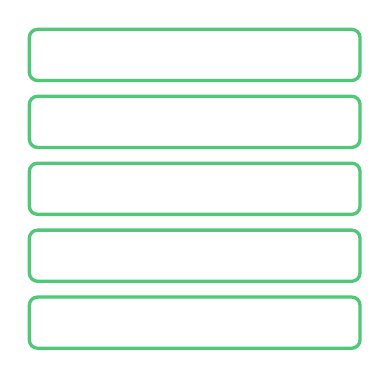
\begin{tikzpicture}[font=\footnotesize]
        \draw[codegreen, line width=1.2pt, rounded corners=3pt] (0,3.525) rectangle (4.2,4.175);
        \node[text=white, font=\footnotesize] at (2.1,3.85) {\checkmark\ \ IoT Sensors};
        \draw[codegreen, line width=1.2pt, rounded corners=3pt] (0,2.675) rectangle (4.2,3.325);
        \node[text=white, font=\footnotesize] at (2.1,3.00) {\checkmark\ \ Embedded Firmware};
        \draw[codegreen, line width=1.2pt, rounded corners=3pt] (0,1.825) rectangle (4.2,2.475);
        \node[text=white, font=\footnotesize] at (2.1,2.15) {\checkmark\ \ Cloud Analytics};
        \draw[codegreen, line width=1.2pt, rounded corners=3pt] (0,0.975) rectangle (4.2,1.625);
        \node[text=white, font=\footnotesize] at (2.1,1.30) {\checkmark\ \ Safety Algorithms};
        \draw[codegreen, line width=1.2pt, rounded corners=3pt] (0,0.125) rectangle (4.2,0.775);
        \node[text=white, font=\footnotesize] at (2.1,0.45) {\checkmark\ \ Healthcare Use-Case};
      \end{tikzpicture}
      \vspace{0.4em}

      \textbf{\textcolor{nithgold}{\small Top 1\% IoT Project}}\\[2pt]
      \textcolor{codegray}{\tiny All pillars successfully implemented}
      \end{center}
    \end{column}
  \end{columns}
\end{frame}

%% ═════════════════════════════════════════
%%  13 — REFERENCES
%% ═════════════════════════════════════════
\begin{frame}[shrink=3]{References}
  \begin{columns}[T]
    \begin{column}{0.5\textwidth}
      \textbf{\textcolor{darkred}{Simulation \& Hardware}}
      \begin{itemize}\setlength\itemsep{0.35em}
        \item \textbf{Wokwi Reference}\\
          {\footnotesize \url{https://wokwi.com}\\
          ESP32 DevKit C v4 docs, DHT22 component, potentiometer simulation guide}

        \item \textbf{ESP32 Reference}\\
          {\footnotesize \url{https://docs.espressif.com}\\
          Technical Reference Manual, ADC1 GPIO specs, WiFi + HTTPClient library}

        \item \textbf{MPU6050 Datasheet}\\
          {\footnotesize InvenSense MPU-6000/6050 Product Spec.\ Rev.\ 3.4}

        \item \textbf{MQ-135 Datasheet}\\
          {\footnotesize Hanwei Electronics MQ-135 Gas Sensor datasheet}
      \end{itemize}
    \end{column}
    \begin{column}{0.5\textwidth}
      \textbf{\textcolor{darkred}{Libraries, Cloud \& Standards}}
      \begin{itemize}\setlength\itemsep{0.35em}
        \item \textbf{DHTesp Library}\\
          {\footnotesize Bernd Giesecke \texttt{beegee-tokyo/DHTesp} (GitHub)}

        \item \textbf{ThingSpeak Platform}\\
          {\footnotesize \url{https://thingspeak.com}\\
          MathWorks REST API documentation}

        \item \textbf{Chart.js Library}\\
          {\footnotesize \url{https://chartjs.org} --- v4.4.4\\
          Open-source charting for real-time dashboards}

        \item \textbf{WHO Cold-Chain Standard}\\
          {\footnotesize WHO Guidelines on Vaccine Cold Chain, WHO/IVB/06.10}

        \item \textbf{DHT22 Datasheet}\\
          {\footnotesize Aosong Electronics AM2302 datasheet}
      \end{itemize}
    \end{column}
  \end{columns}
\end{frame}

%% ═════════════════════════════════════════
%%  THANK YOU
%% ═════════════════════════════════════════
\begin{frame}
  \begin{center}
    \vspace{1.2cm}
    \textbf{\textcolor{darkred}{\Huge Thank You}}

    \vspace{0.7cm}
    \textcolor{nithgold}{\large Questions \& Discussion}

    \vspace{0.9cm}
    {\small
    \textbf{Anirudh Sharma} $|$ Roll No: 22DCS002\\
    BTech DD 8\textsuperscript{th} Semester, 2025--26\\[0.3em]
    \textcolor{codegray}{Department of Computer Science and Engineering}\\
    \textcolor{codegray}{National Institute of Technology Hamirpur}
    }

    \vspace{0.7cm}
    
\includegraphics[height=1.5cm]{nith_logo.png}
  \end{center}
\end{frame}

\end{document}
